\documentclass{standalone}
\usepackage{graphicx}	
\usepackage{amssymb, amsmath}
\usepackage{color}

\usepackage{tikz}
\usetikzlibrary{intersections, backgrounds, math}
\usepackage{pgfmath}

\definecolor{light}{RGB}{220, 188, 188}
\definecolor{mid}{RGB}{185, 124, 124}
\definecolor{dark}{RGB}{143, 39, 39}
\definecolor{highlight}{RGB}{180, 31, 180}
\definecolor{gray10}{gray}{0.1}
\definecolor{gray20}{gray}{0.2}
\definecolor{gray30}{gray}{0.3}
\definecolor{gray40}{gray}{0.4}
\definecolor{gray60}{gray}{0.6}
\definecolor{gray70}{gray}{0.7}
\definecolor{gray80}{gray}{0.8}
\definecolor{gray90}{gray}{0.9}
\definecolor{gray95}{gray}{0.95}


\begin{document}

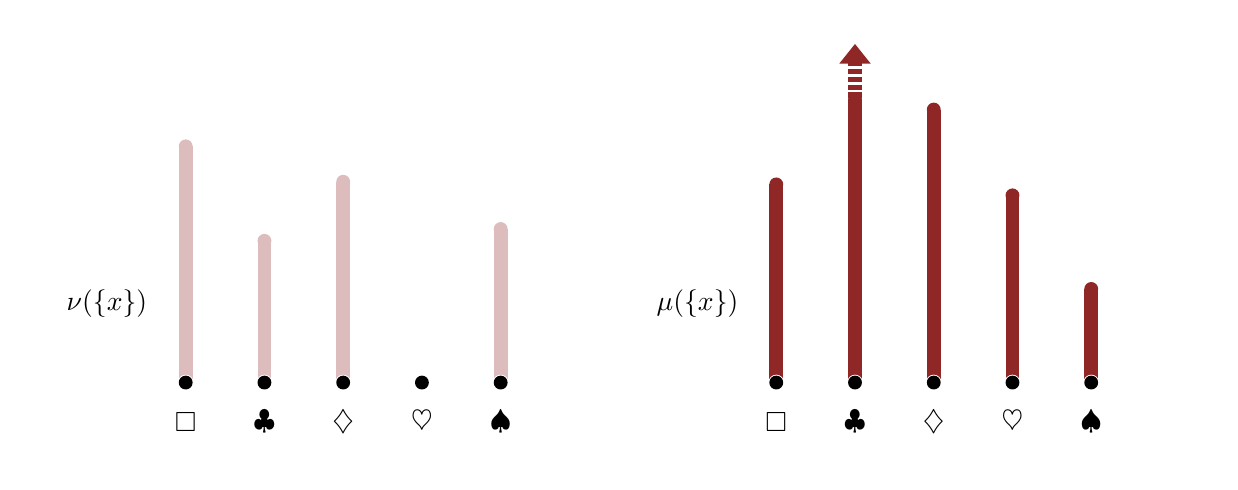
\begin{tikzpicture}[scale=1]
  \begin{scope}[shift={(0, 0)}]
    \draw[white] (-4, -3) rectangle (3.5, 2.5);
    
    \foreach [count=\n] \m in {0.2, 0.12, 0.17, 0, 0.13} {
      \pgfmathsetmacro{\x}{1.0 * ( (\n - 1) - 2)};
      \draw[light, line width=5] (\x, -2) -- (\x, {(15 * \m - 2)});
      \fill[light] (\x, {(15 * \m - 2)}) circle (0.088);
      \fill[white] (\x, -2) circle (0.1);
      \fill[black] (\x, -2) circle (0.088);
    }
    
    \node at (-2, -2.5) { $\Box$ };
    \node at (-1, -2.5) { $\clubsuit$ };
    \node at (0, -2.5) { $\diamondsuit$ };
    \node at (1, -2.5) { $\heartsuit$ };
    \node at (2, -2.5) { $\spadesuit$ };
 
    \node at (-3, -1) { $\nu( \{ x \} )$ };
  \end{scope}
  
\begin{scope}[shift={(7.5, 0)}]
    \draw[white] (-4, -3) rectangle (3.5, 2.5);
    
    \foreach [count=\n] \m in {0.167790, 0.239700, 0.231140, 0.158496, 0.079248} {
      \pgfmathsetmacro{\x}{1.0 * ( (\n - 1) - 2)};
      \draw[dark, line width=5] (\x, -2) -- (\x, {(15 * \m - 2)});
      \fill[dark] (\x, {(15 * \m - 2)}) circle (0.088);
      \fill[white] (\x, -2) circle (0.1);
      \fill[black] (\x, -2) circle (0.088);
    }
    
    \foreach \n in {0, 1, ..., 5} {
      \pgfmathsetmacro{\y}{0.1 * (\n - 1) + 1.75};
      \draw[dark, line width=2] (-1 - 0.088, \y) -- (-1 + 0.088, \y);
    }
    \fill[dark] (-1 - 0.2, 2.05) -- (-1, 2.3) -- (-1 + 0.2, 2.05) -- cycle;
    
    \node at (-2, -2.5) { $\Box$ };
    \node at (-1, -2.5) { $\clubsuit$ };
    \node at (0, -2.5) { $\diamondsuit$ };
    \node at (1, -2.5) { $\heartsuit$ };
    \node at (2, -2.5) { $\spadesuit$ };
 
    \node at (-3, -1) { $\mu( \{ x \} )$ };
  \end{scope}
  
\end{tikzpicture}

\end{document}  